\documentclass[../main.tex]{subfiles}

\begin{document}
\chapter{Einführung}\label{chp:real}
\section{Ziele der Vorlesung}
\begin{goals}
  \begin{itemize}
    \item Addieren, Speichern, Berechnen \newline
      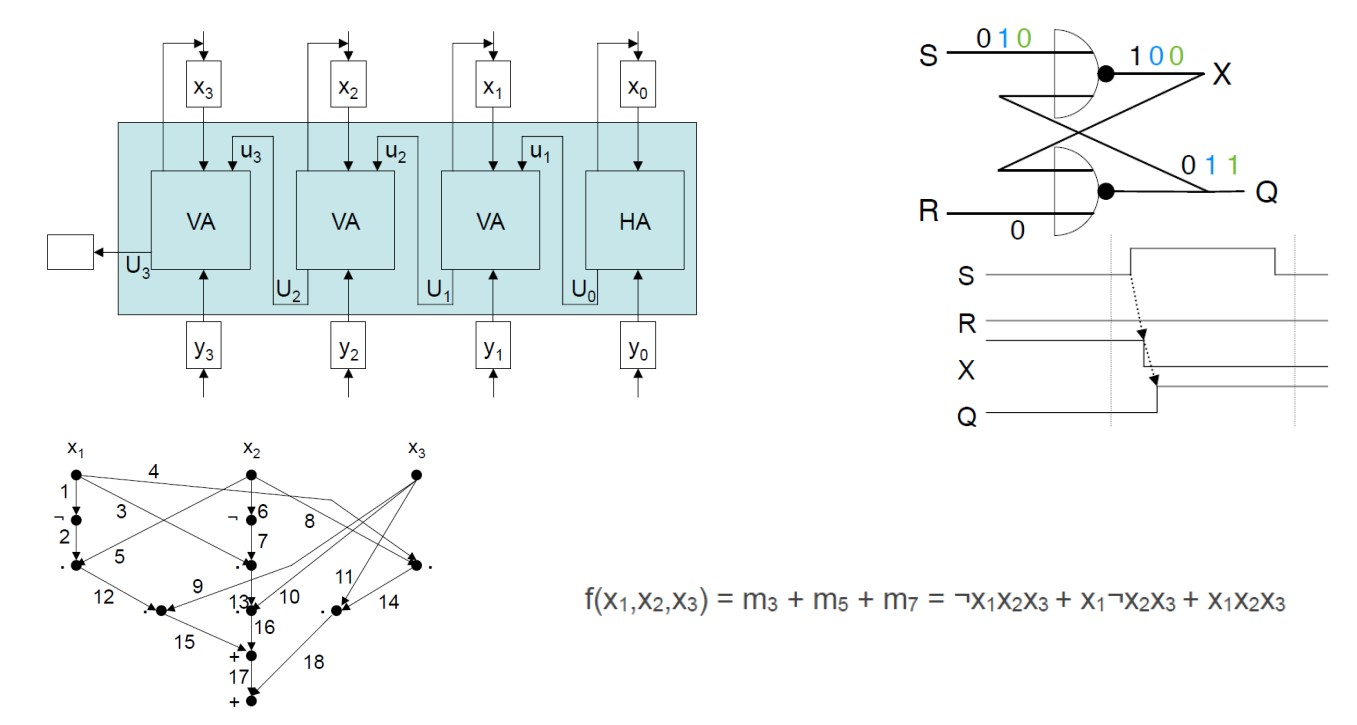
\includegraphics[height=5cm]{01-addieren}
    \item Arithmetic Logic Unit \newline
      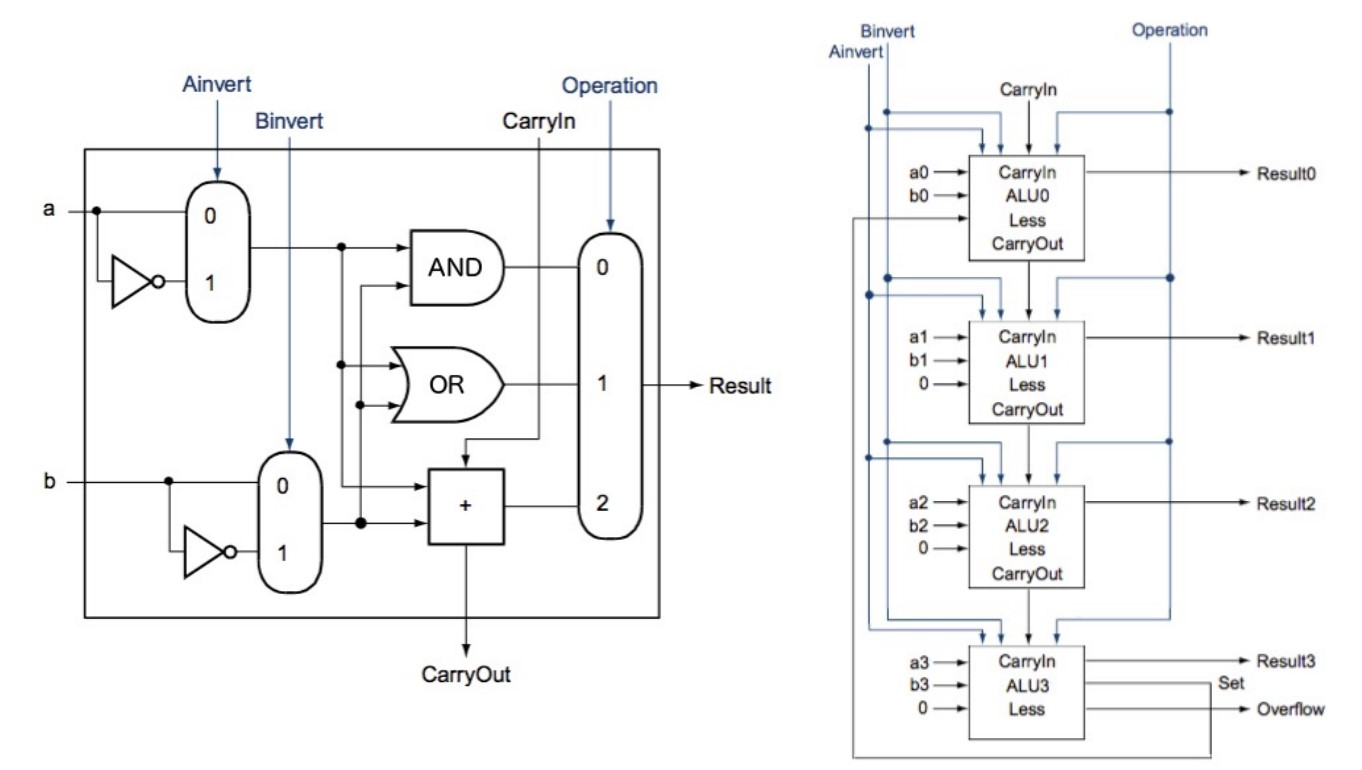
\includegraphics[height=5cm]{01-ALU}
    \item Literatur\newline
      
\includegraphics[height=5cm]{01-Books}
    \item Diskrete Mathematik
      \begin{itemize}
      \item[">] Es wird ein paar inhaltliche Überschneidungen zwischen GTI
      und der Vorlesung Diskrete Mathematik geben
      \item[">]Dies betrifft vor allem die nächsten beiden Kapitel
      \item[">]Verwenden Sie in GTI die Definitionen aus der GTI Vorlesung
      und in DM diejenigen aus der DM Vorlesung
      \end{itemize}
  \end{itemize}
\end{goals}
\section{Geschichte}
Wen's interessiert soll die slides durchschauen oder eine Zusammenfassung davon schreiben, da sie aber wahrscheinlich nicht
Prüfungsrelevant ist, behandle ich die hier kaum. 
\subsection{Moore's Law}
\label{subsec:moore's_law}{}
\begin{moore_law}
  Das Mooresche Gesetz (englisch Moore’s law; deutsch „Gesetz“ im Sinne von „Gesetzmäßigkeit“) besagt, 
  dass sich die Komplexität integrierter Schaltkreise mit minimalen Komponentenkosten regelmäßig verdoppelt; 
  je nach Quelle werden 12, 18 oder 24 Monate als Zeitraum genannt. Unter Komplexität verstand Gordon Moore, 
  der das Gesetz 1965 formulierte, die Anzahl der Schaltkreiskomponenten auf einem integrierten Schaltkreis. Gelegentlich 
  ist auch von einer Verdoppelung der Integrationsdichte die Rede, also der Anzahl an Transistoren pro Flächeneinheit. 
  Diese technische Entwicklung bildet eine wesentliche Grundlage der „digitalen Revolution“.
  \newline
  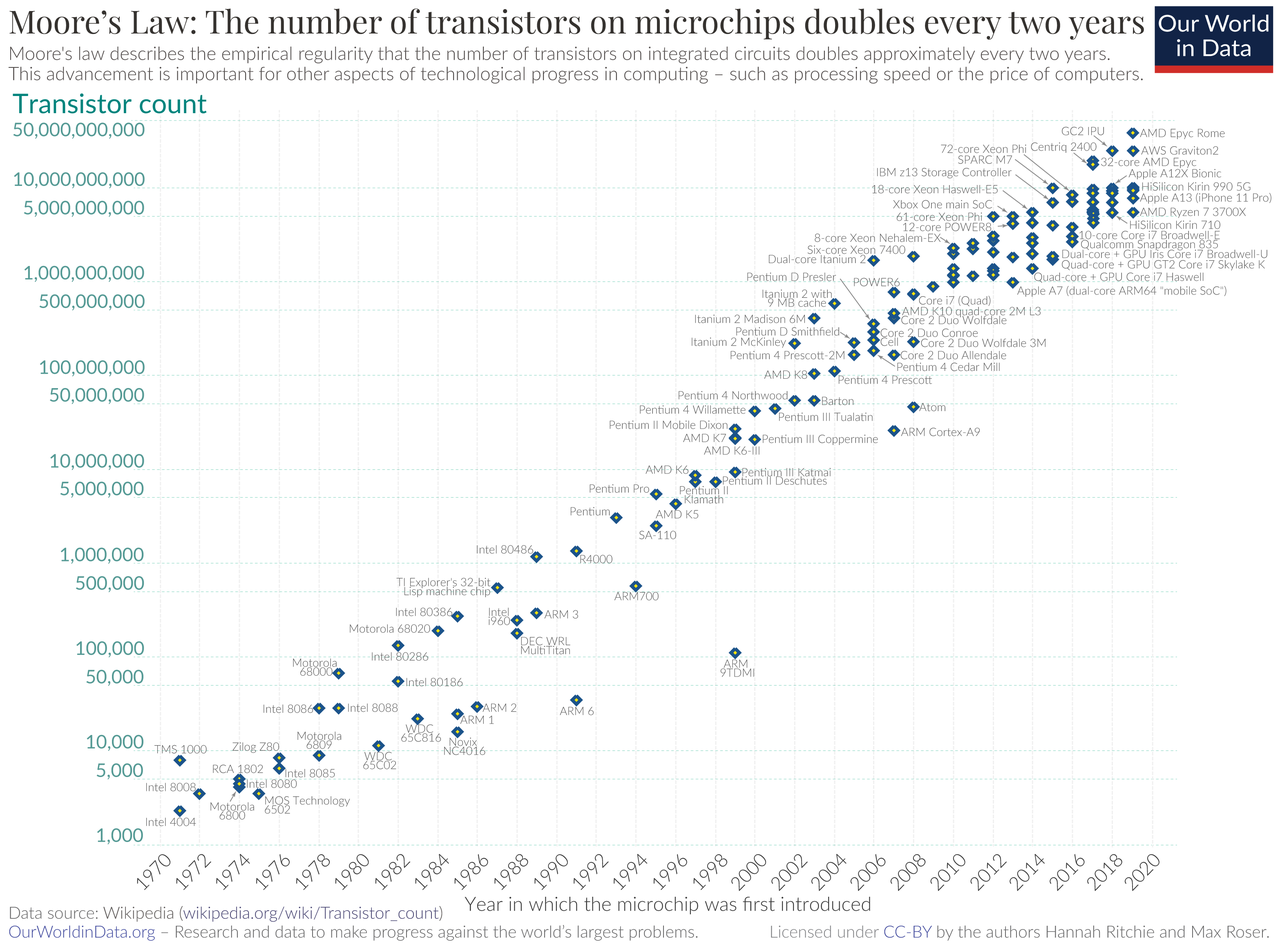
\includegraphics[width=\textwidth]{01-Moore_law}
\end{moore_law}
Quelle: https://de.wikipedia.org/wiki/Mooresches\_Gesetz
\subsection{Koomey's Law}
\label{subsec:koomey's_law}
\begin{koomey_law}{}
  Das Koomey-Gesetz beschreibt einen Trend in der Geschichte der Computerhardware: Etwa ein halbes Jahrhundert 
  lang verdoppelte sich die Zahl der Berechnungen pro Joule verbrauchter Energie etwa alle 1,57 Jahre. 
  Professor Jonathan Koomey beschrieb diesen Trend in einem Papier aus dem Jahr 2010, in dem er schrieb, 
  dass "bei einer festen Rechenlast die benötigte Batteriemenge alle anderthalb Jahre um den Faktor zwei abnimmt".

  Dieser Trend war seit den 1950er Jahren bemerkenswert stabil gewesen ($R^2$ von über 98 \%)
  Im Jahr 2011 untersuchte Koomey diese Daten jedoch erneut und stellte fest, dass sich die Verdopplung nach dem Jahr 2000 
  auf etwa alle 2,6 Jahre verlangsamte. Dies hängt mit der Verlangsamung des Mooreschen Gesetzes$^{\ref{subsec:moore's_law}}$ 
  zusammen, also der Möglichkeit, kleinere Transistoren zu bauen, und mit dem Ende der Dennard-Skalierung um 2005, 
  also der Möglichkeit, kleinere Transistoren mit konstanter Leistungsdichte zu bauen.

  "Der Unterschied zwischen diesen beiden Wachstumsraten ist beträchtlich. Eine Verdopplung alle anderthalb 
  Jahre führt zu einer 100-fachen Steigerung der Effizienz pro Jahrzehnt. Eine Verdopplung alle zweieinhalb 
  Jahre ergibt nur eine 16-fache Steigerung", schrieb Koomey.
  \newline
  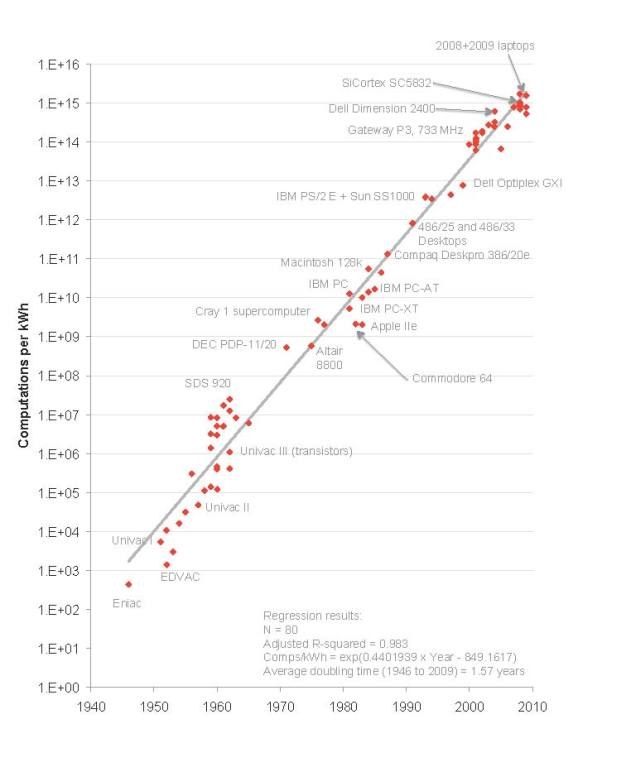
\includegraphics[width=\textwidth]{01-koomey_law}
\end{koomey_law}
Quelle: https://en.wikipedia.org/wiki/Koomey\%27s\_law
\section{Boolsche Logik}
\subsection{George Boole (1815-1864)}
The Laws of Thought (1854):\newline
Logisches Denken wird auf das Lösen von Gleichungen reduziert.\newline
\begin{flushright}
  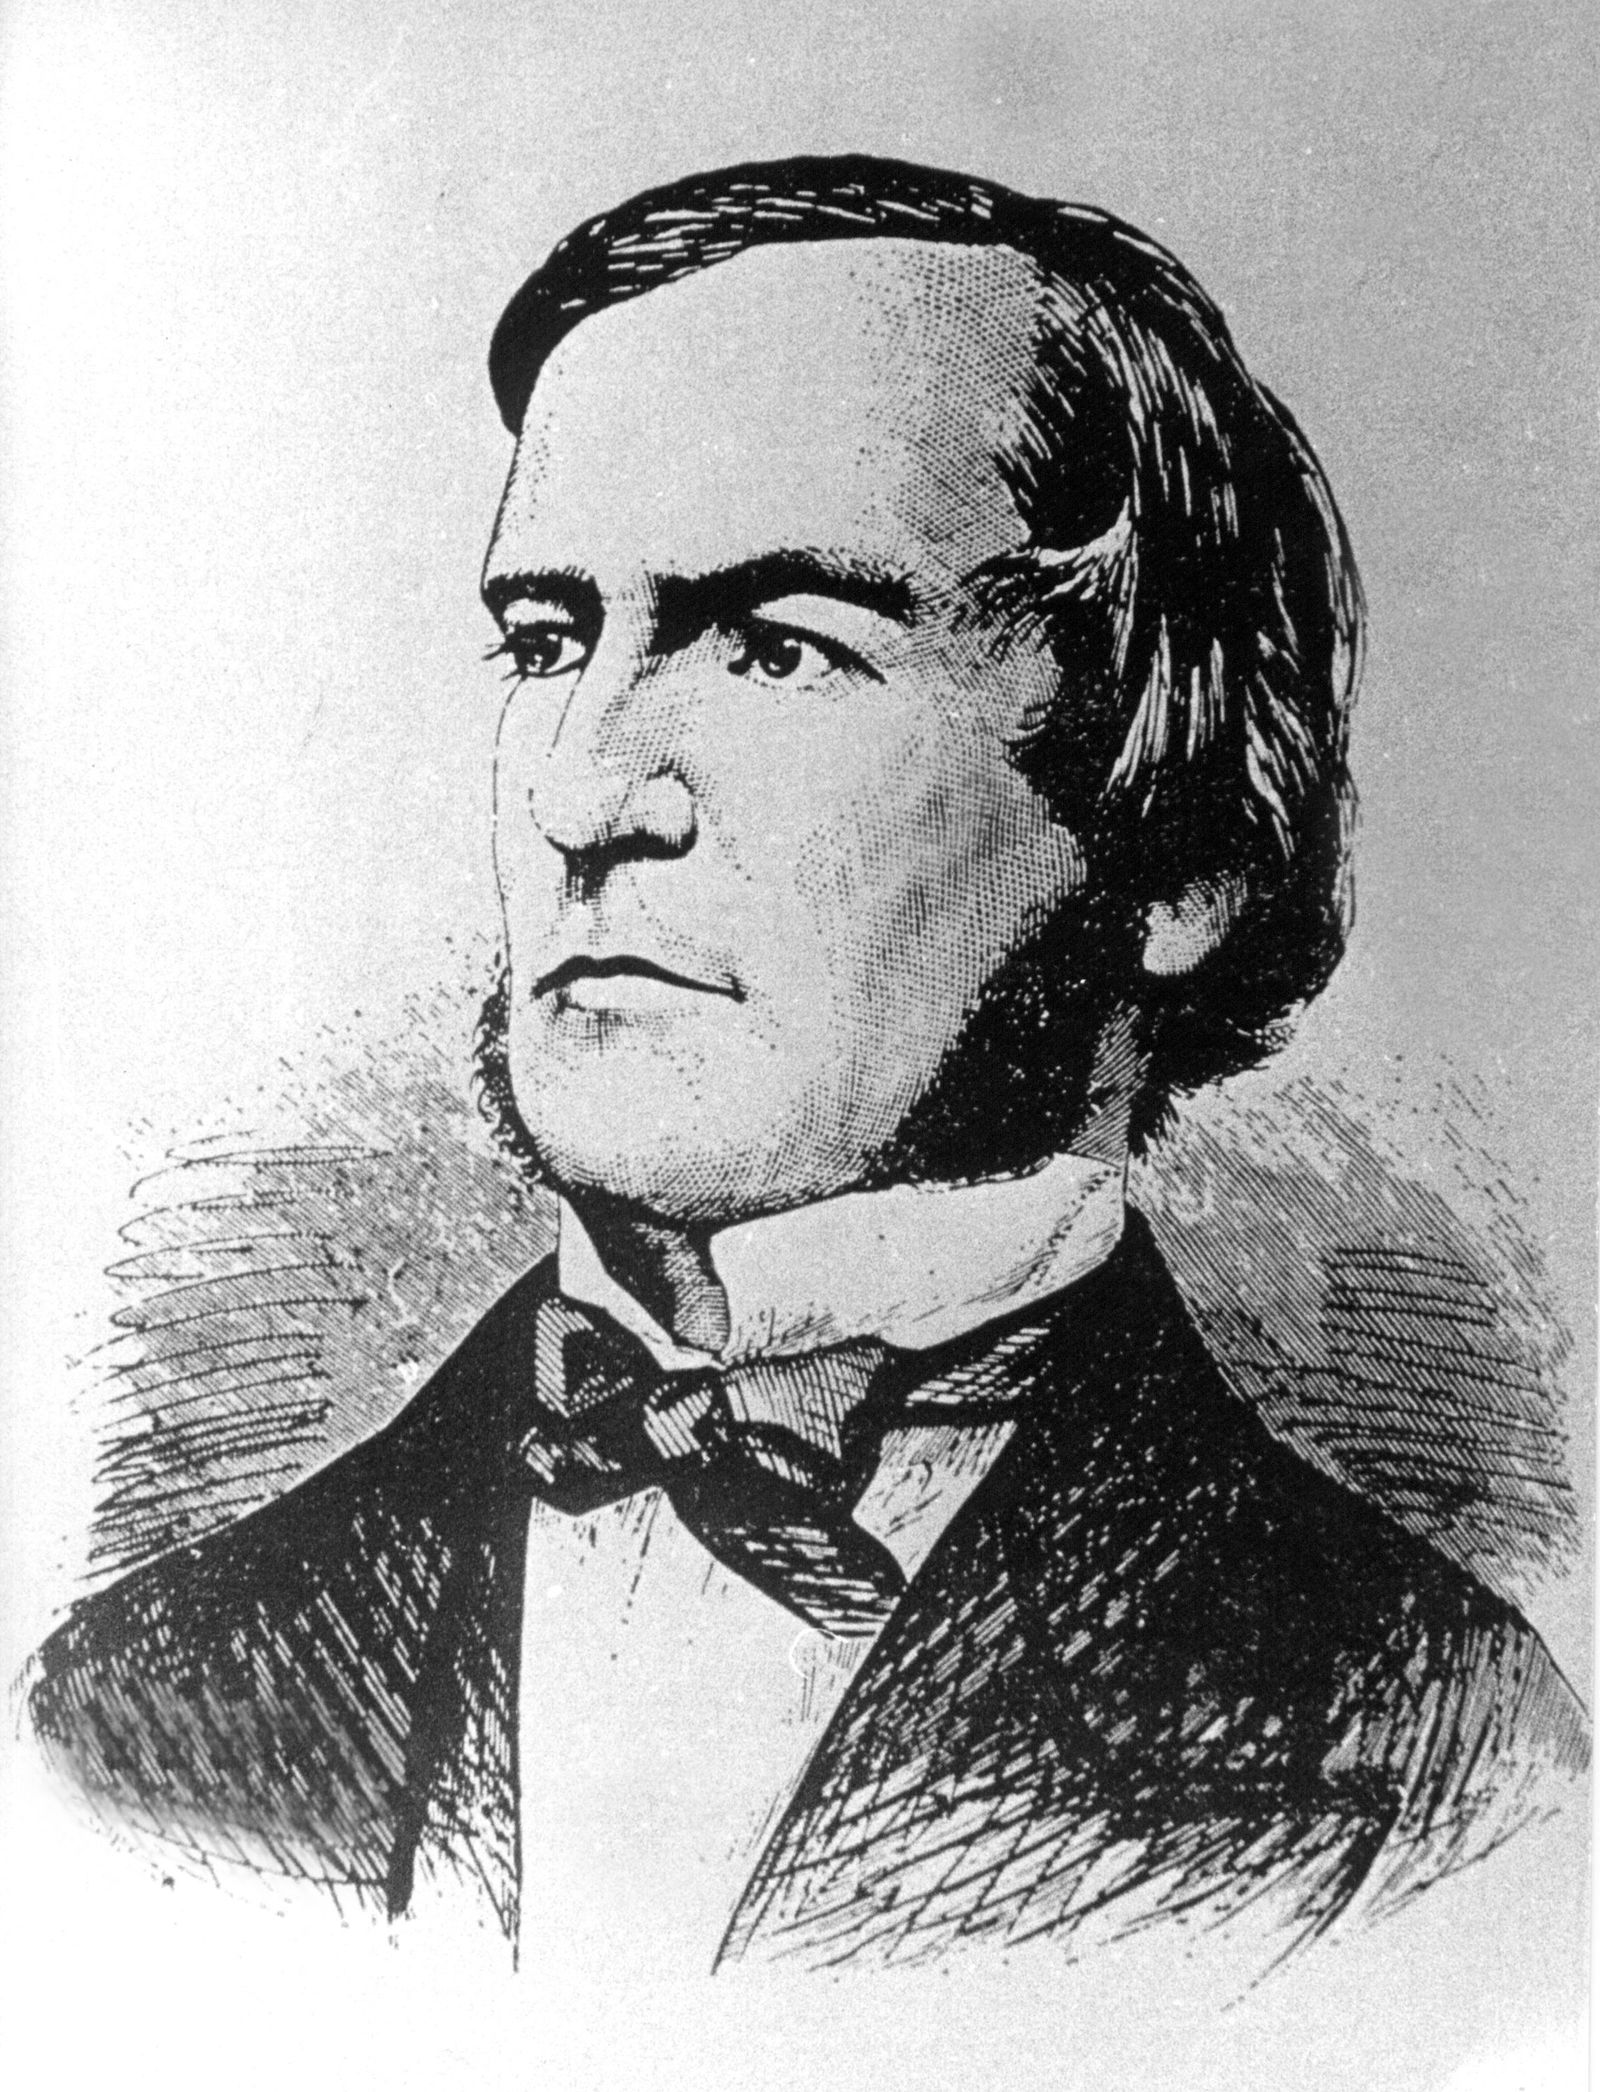
\includegraphics[width=3cm]{01-george_boole}
 \end{flushright}
\subsection{boolsche Logik}
\begin{itemize}
  \item $x, y$ seien Kollektionen von Objekten
  \item $x + y$ ist die Kollektion von allen Objekten, die zu x und 
  zu y gehören (Vereinigung)
  \item $xy$ ist die Kollektion von allen Objekten, die zu x und zu y gehören (Schnitt)
  \item $0$ ist die leere Kollektion
\end{itemize}
\begin{itemize}
  \item Alle s sind p $s = sp$
  \item Kein s ist p $sp = 0$
  \item Einige s sind p $sp \neq 0$
  \item Einige s sind nicht p $s \neq sp$
  \item Rechenregeln: 
  \begin{itemize}
    \item[] $(xy)z = x(yz)$
    \item[] $x0 = 0$
  \end{itemize}
  \begin{example}\newline
      $b$: Berner \newline
      $s$: Schweizer\newline
      $m$: auf dem Mond gewesen\newline\newline

      Alle $b$ sind $s$ = $b = bs$\newline
      Kein $s$ ist $m$ = $sm=0$\newline\newline
      $bm=(bs)m=b(sm)=b0=0$\newline
      Also $bm=0$, also kein $b$ ist $m$
    \end{example}  
\end{itemize}
\end{document}